% ==================================================
% Section 5
% ==================================================
\section{Discrete-Time Adaptive Controller}

Implementation of the adaptive controller on a microcontroller requires a discrete-time ~formulation. In this section, the continuous-time adaptive controller developed in Section~2 is converted using the indirect approach. The controller is first designed in continuous time and then approximated by a discrete-time controller.

\subsection{Discrete-Time Formulation}

The continuous-time controller developed in Section~2 is converted into a discrete-time controller by approximating the error derivatives using backward differences:
\begin{equation}
\dot{e}[k] \approx \frac{e[k]-e[k-1]}{T_s},
\qquad
\ddot{e}[k] \approx \frac{e[k]-2e[k-1]+e[k-2]}{T_s^2}.
\label{eq:discrete_bd}
\end{equation}
The filtered error \(z[k]\), the regressor vector \(\phi[k]\), the auxiliary signal \(y_r^{(3)}[k]\), and the control input \(u[k]\) are then evaluated using the same expressions as in Section~2, with all signals sampled at \(t=kT_s\). The sampling period \(T_s\) is the time between two consecutive control updates. The control input is held constant between samples by a zero-order hold (ZOH):
\begin{equation}
u(t) = u[k], \qquad kT_s \le t < (k+1)T_s.
\end{equation}
The adaptation law is converted into a discrete-time update:
\begin{equation}
\hat{\theta}[k+1]
=
\hat{\theta}[k]
-
T_s\,\Gamma\,\phi[k]\,z[k].
\label{eq:discrete_adaptation_law}
\end{equation}
This recursive equation can be implemented directly on a microcontroller by updating the parameter estimates once every sampling period.

\subsection{Simulation Results}

The simulation results are presented in figures~\ref{fig:discrete_tracking}--\ref{fig:zoh_detail}. The discrete-time adaptive controller tracks the reference model output while updating the parameter estimates online.

\begin{figure}[H]
\centering
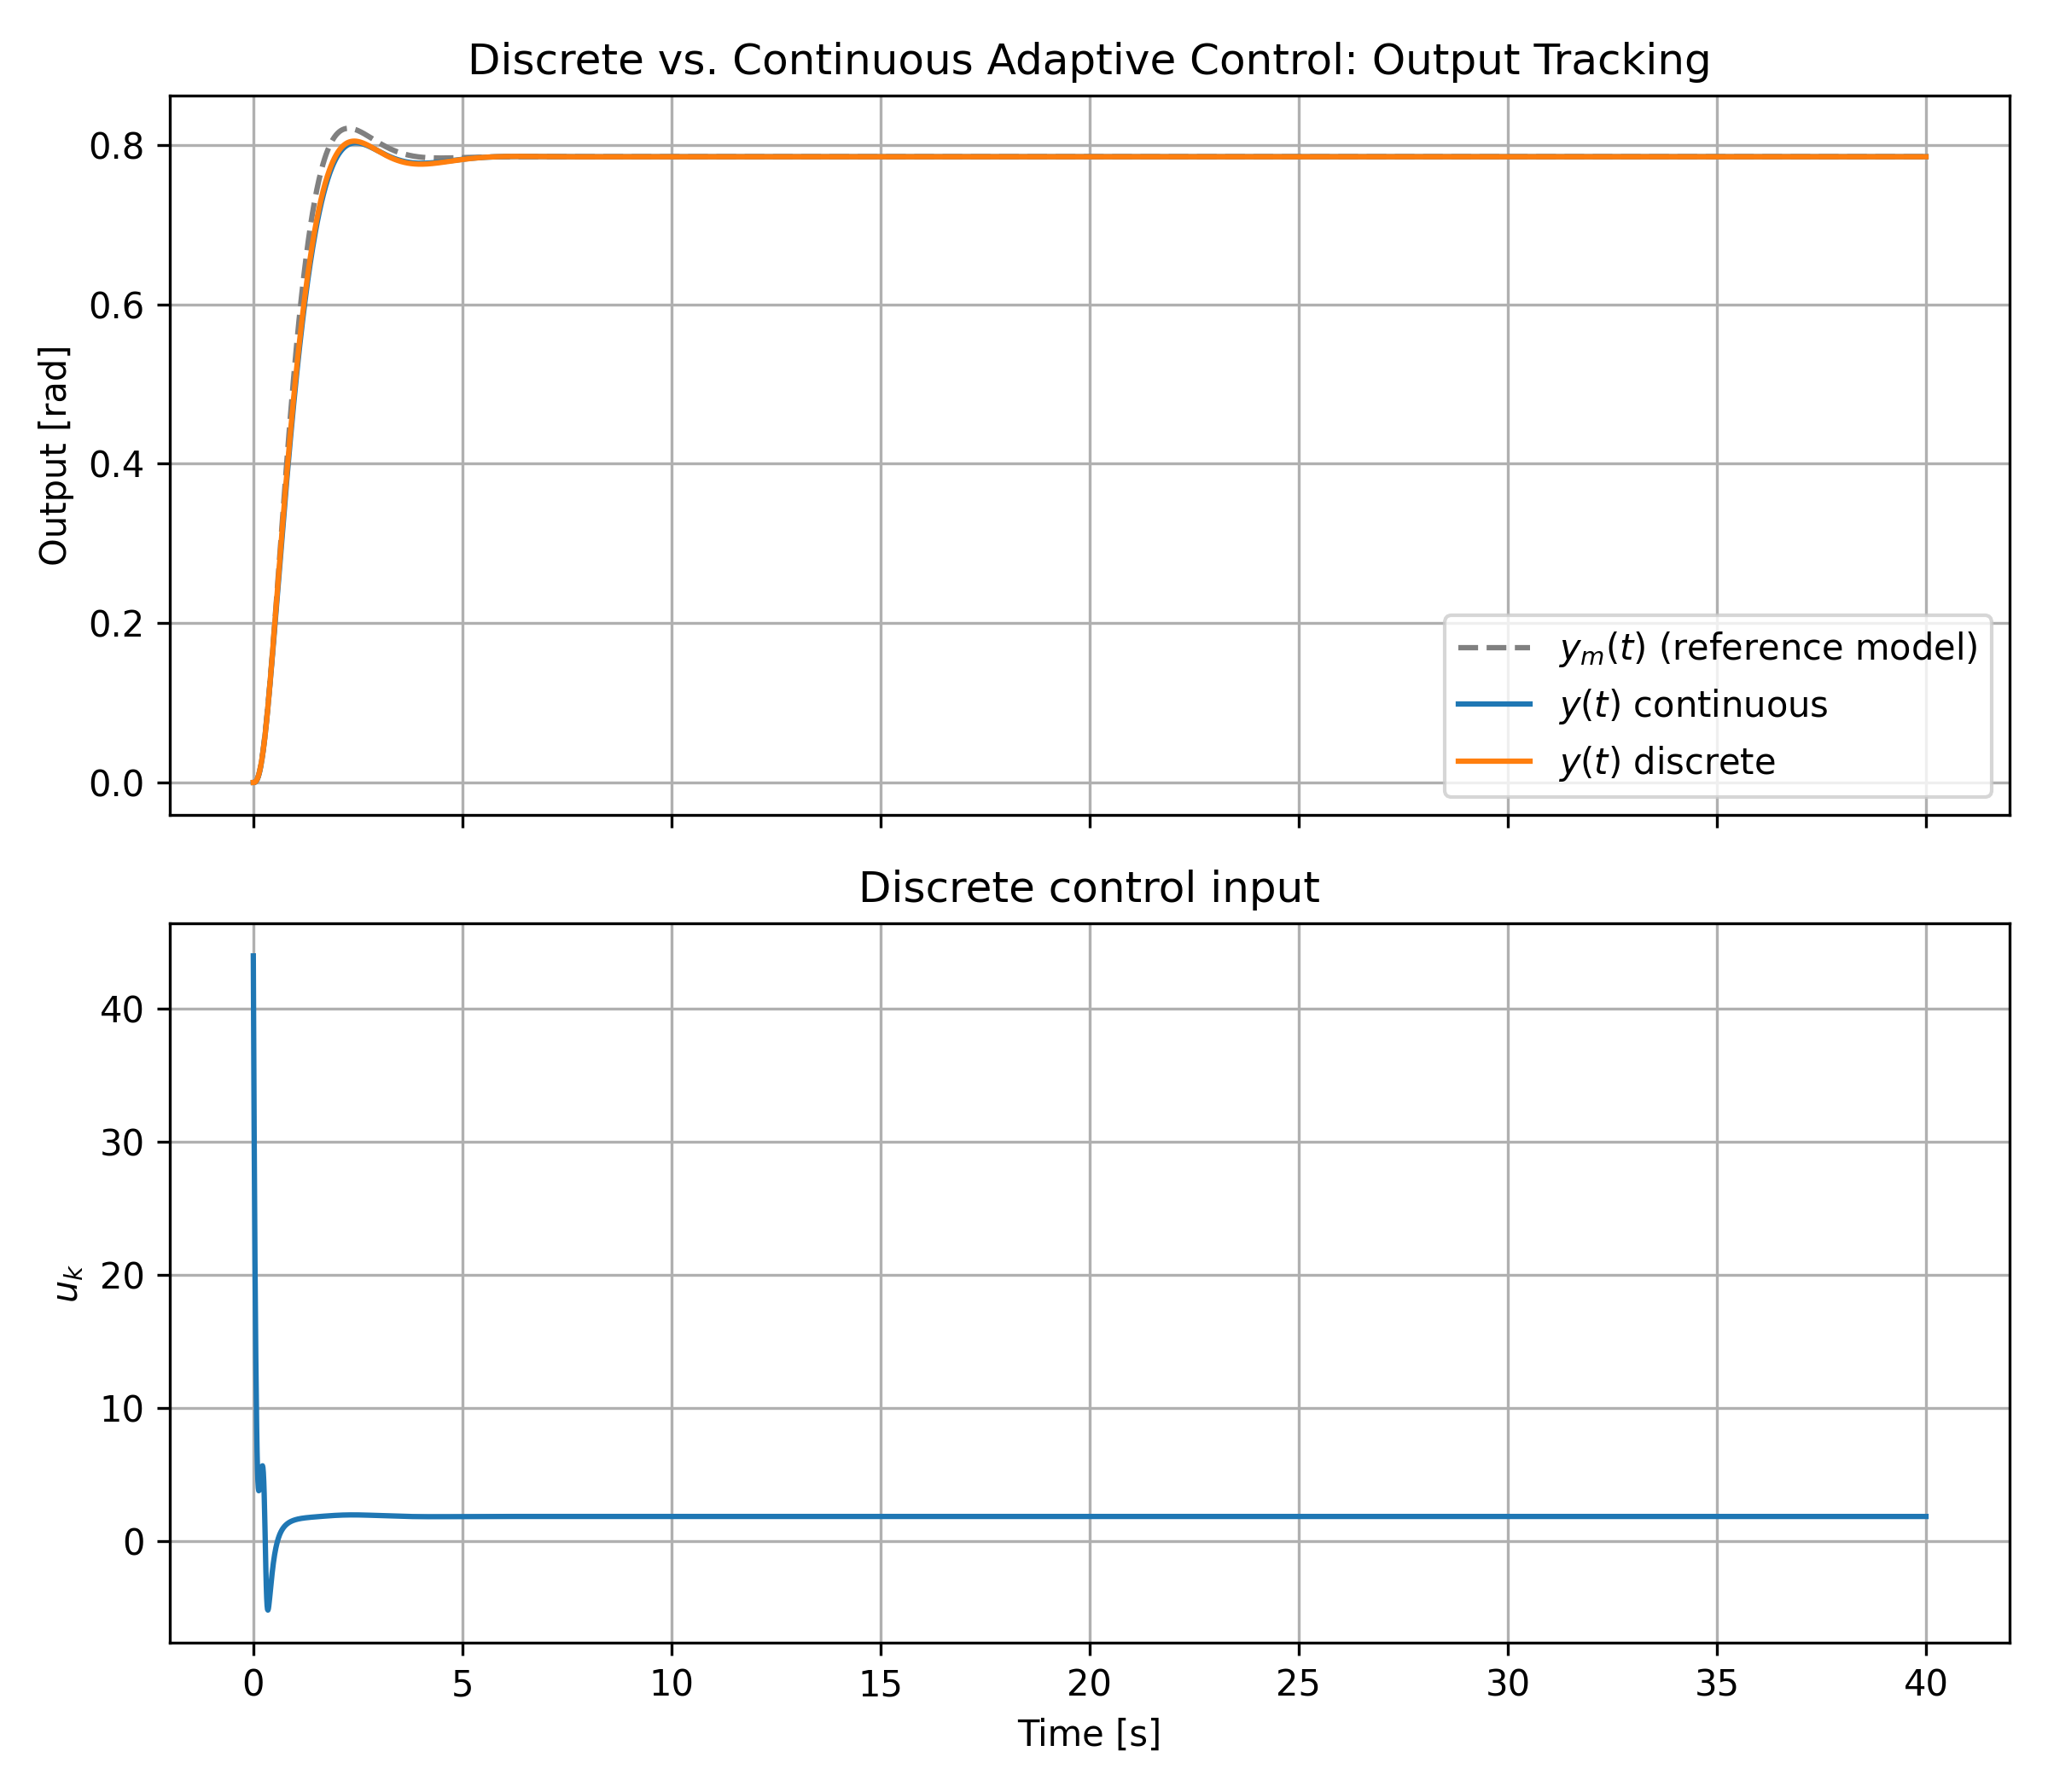
\includegraphics[width=0.7\textwidth]{figs/hw/section5_discrete_vs_continuous_tracking.png}
\caption{Reference model \(y_m(t)\), continuous-time plant output, and discrete-time plant output (top); Discrete control input \(u_k\) (bottom).}
\label{fig:discrete_tracking}
\end{figure}

\begin{figure}[H]
\centering
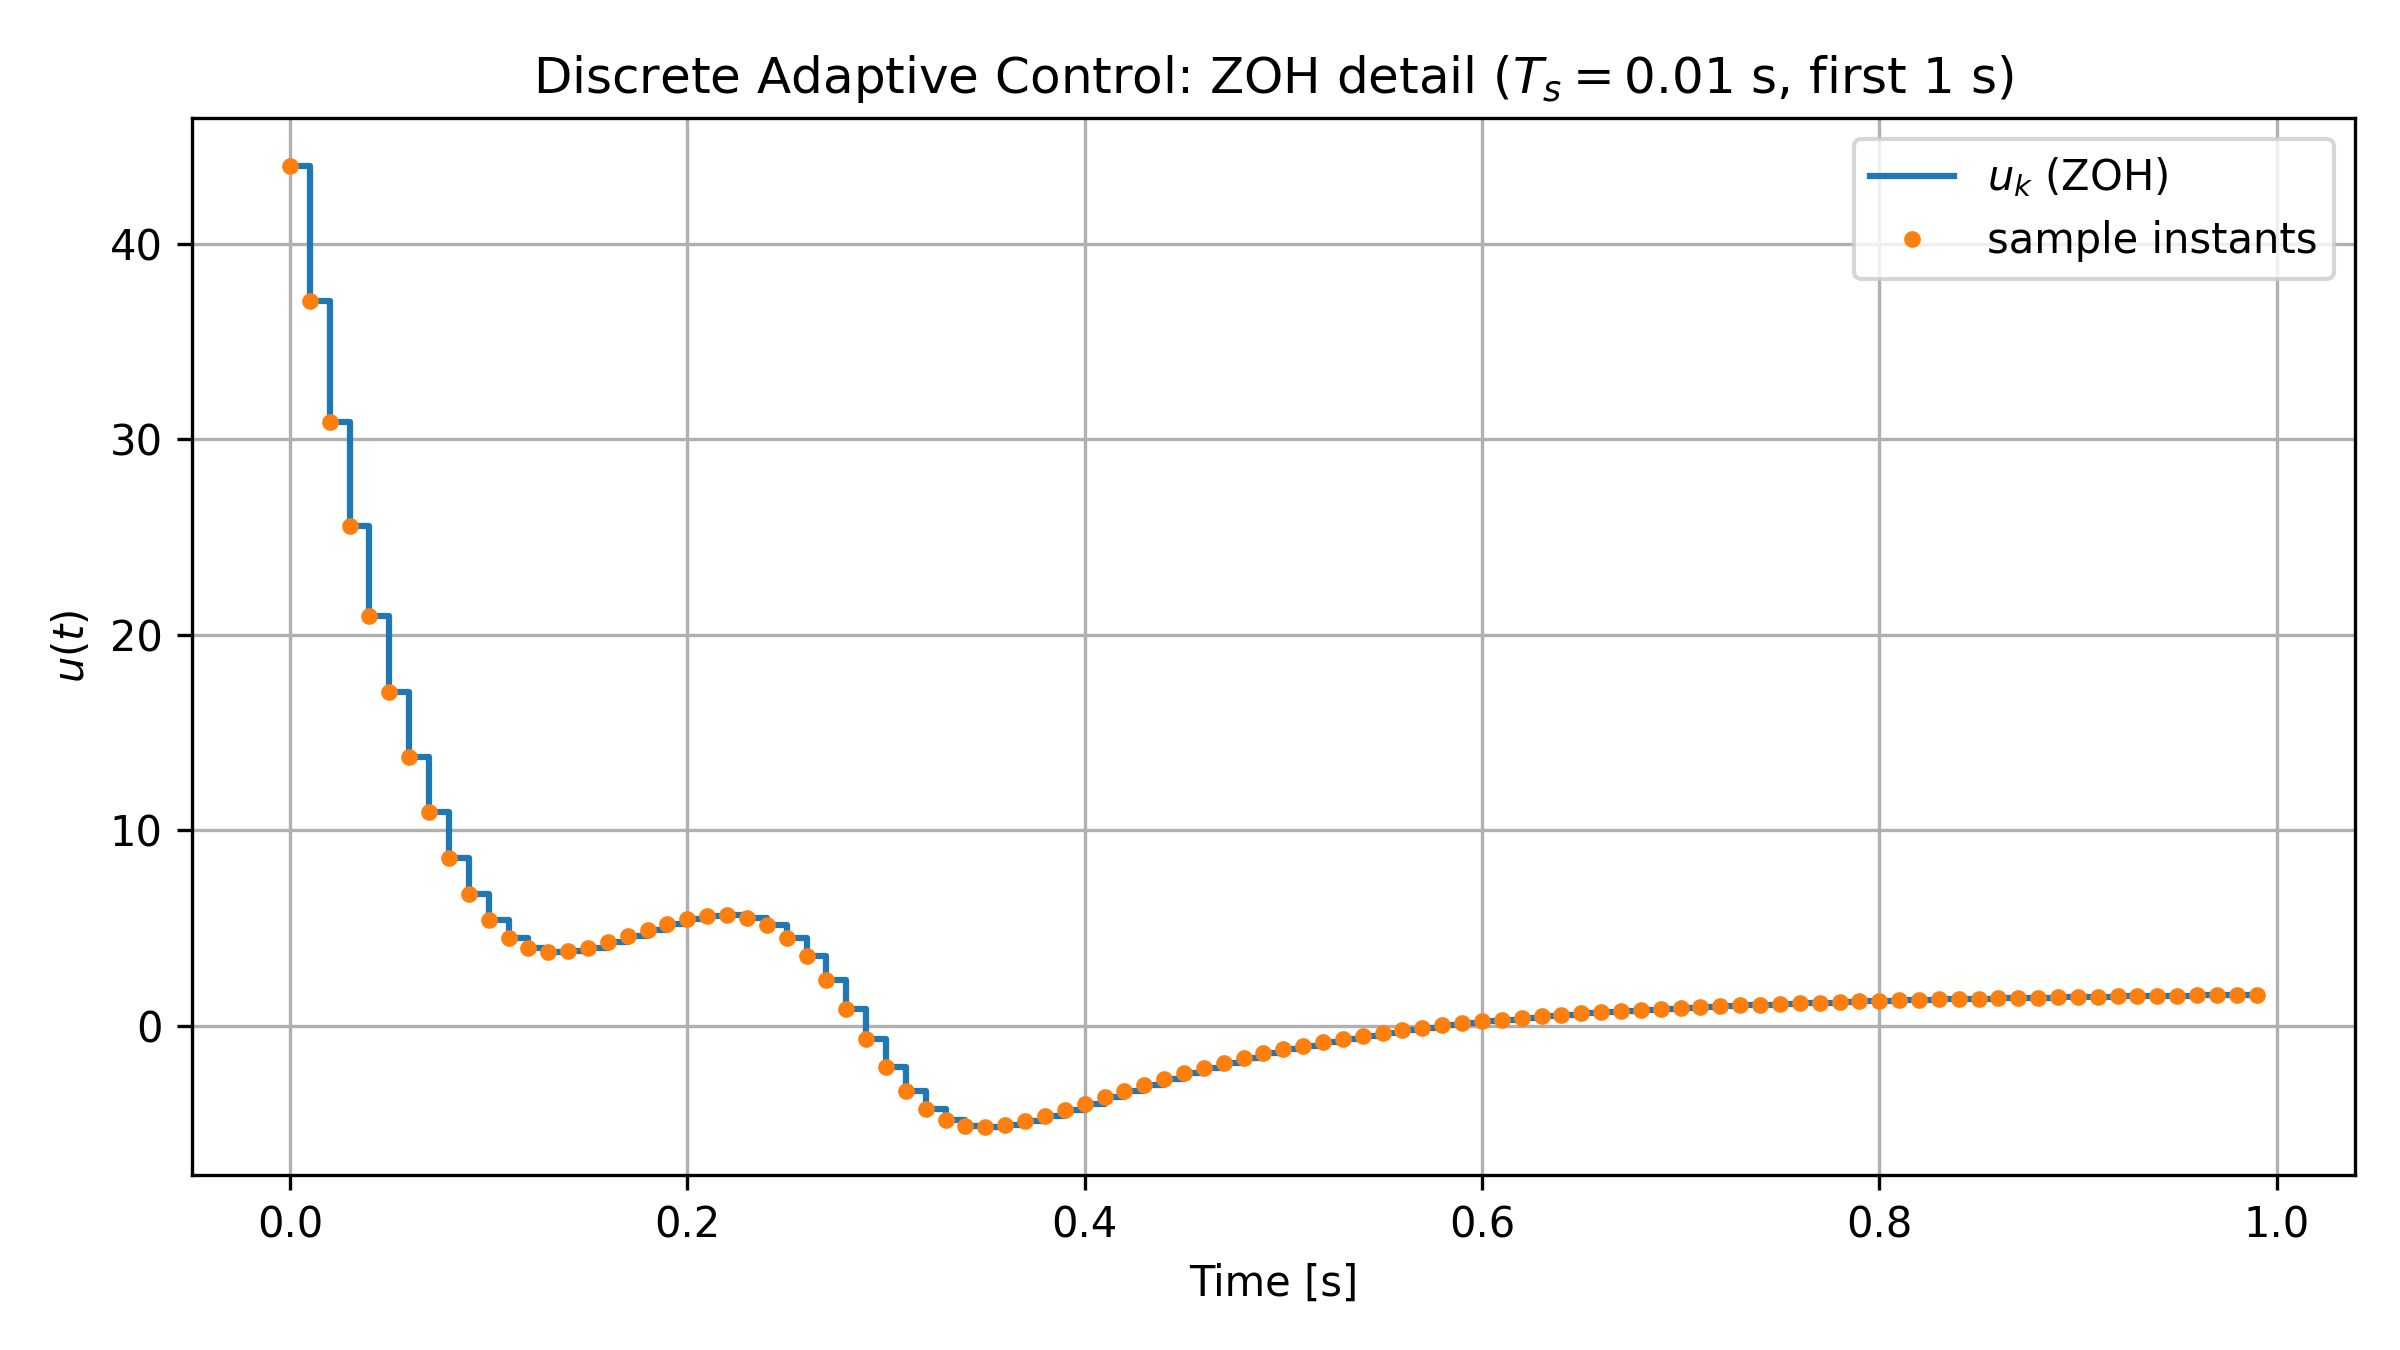
\includegraphics[width=0.7\textwidth]{figs/hw/section5_discrete_u_zoh_detail.png}
\caption{Zoomed view of the digital control input over $0-1s$ of simulation.}
\label{fig:zoh_detail}
\end{figure}

\begin{figure}[H]
\centering
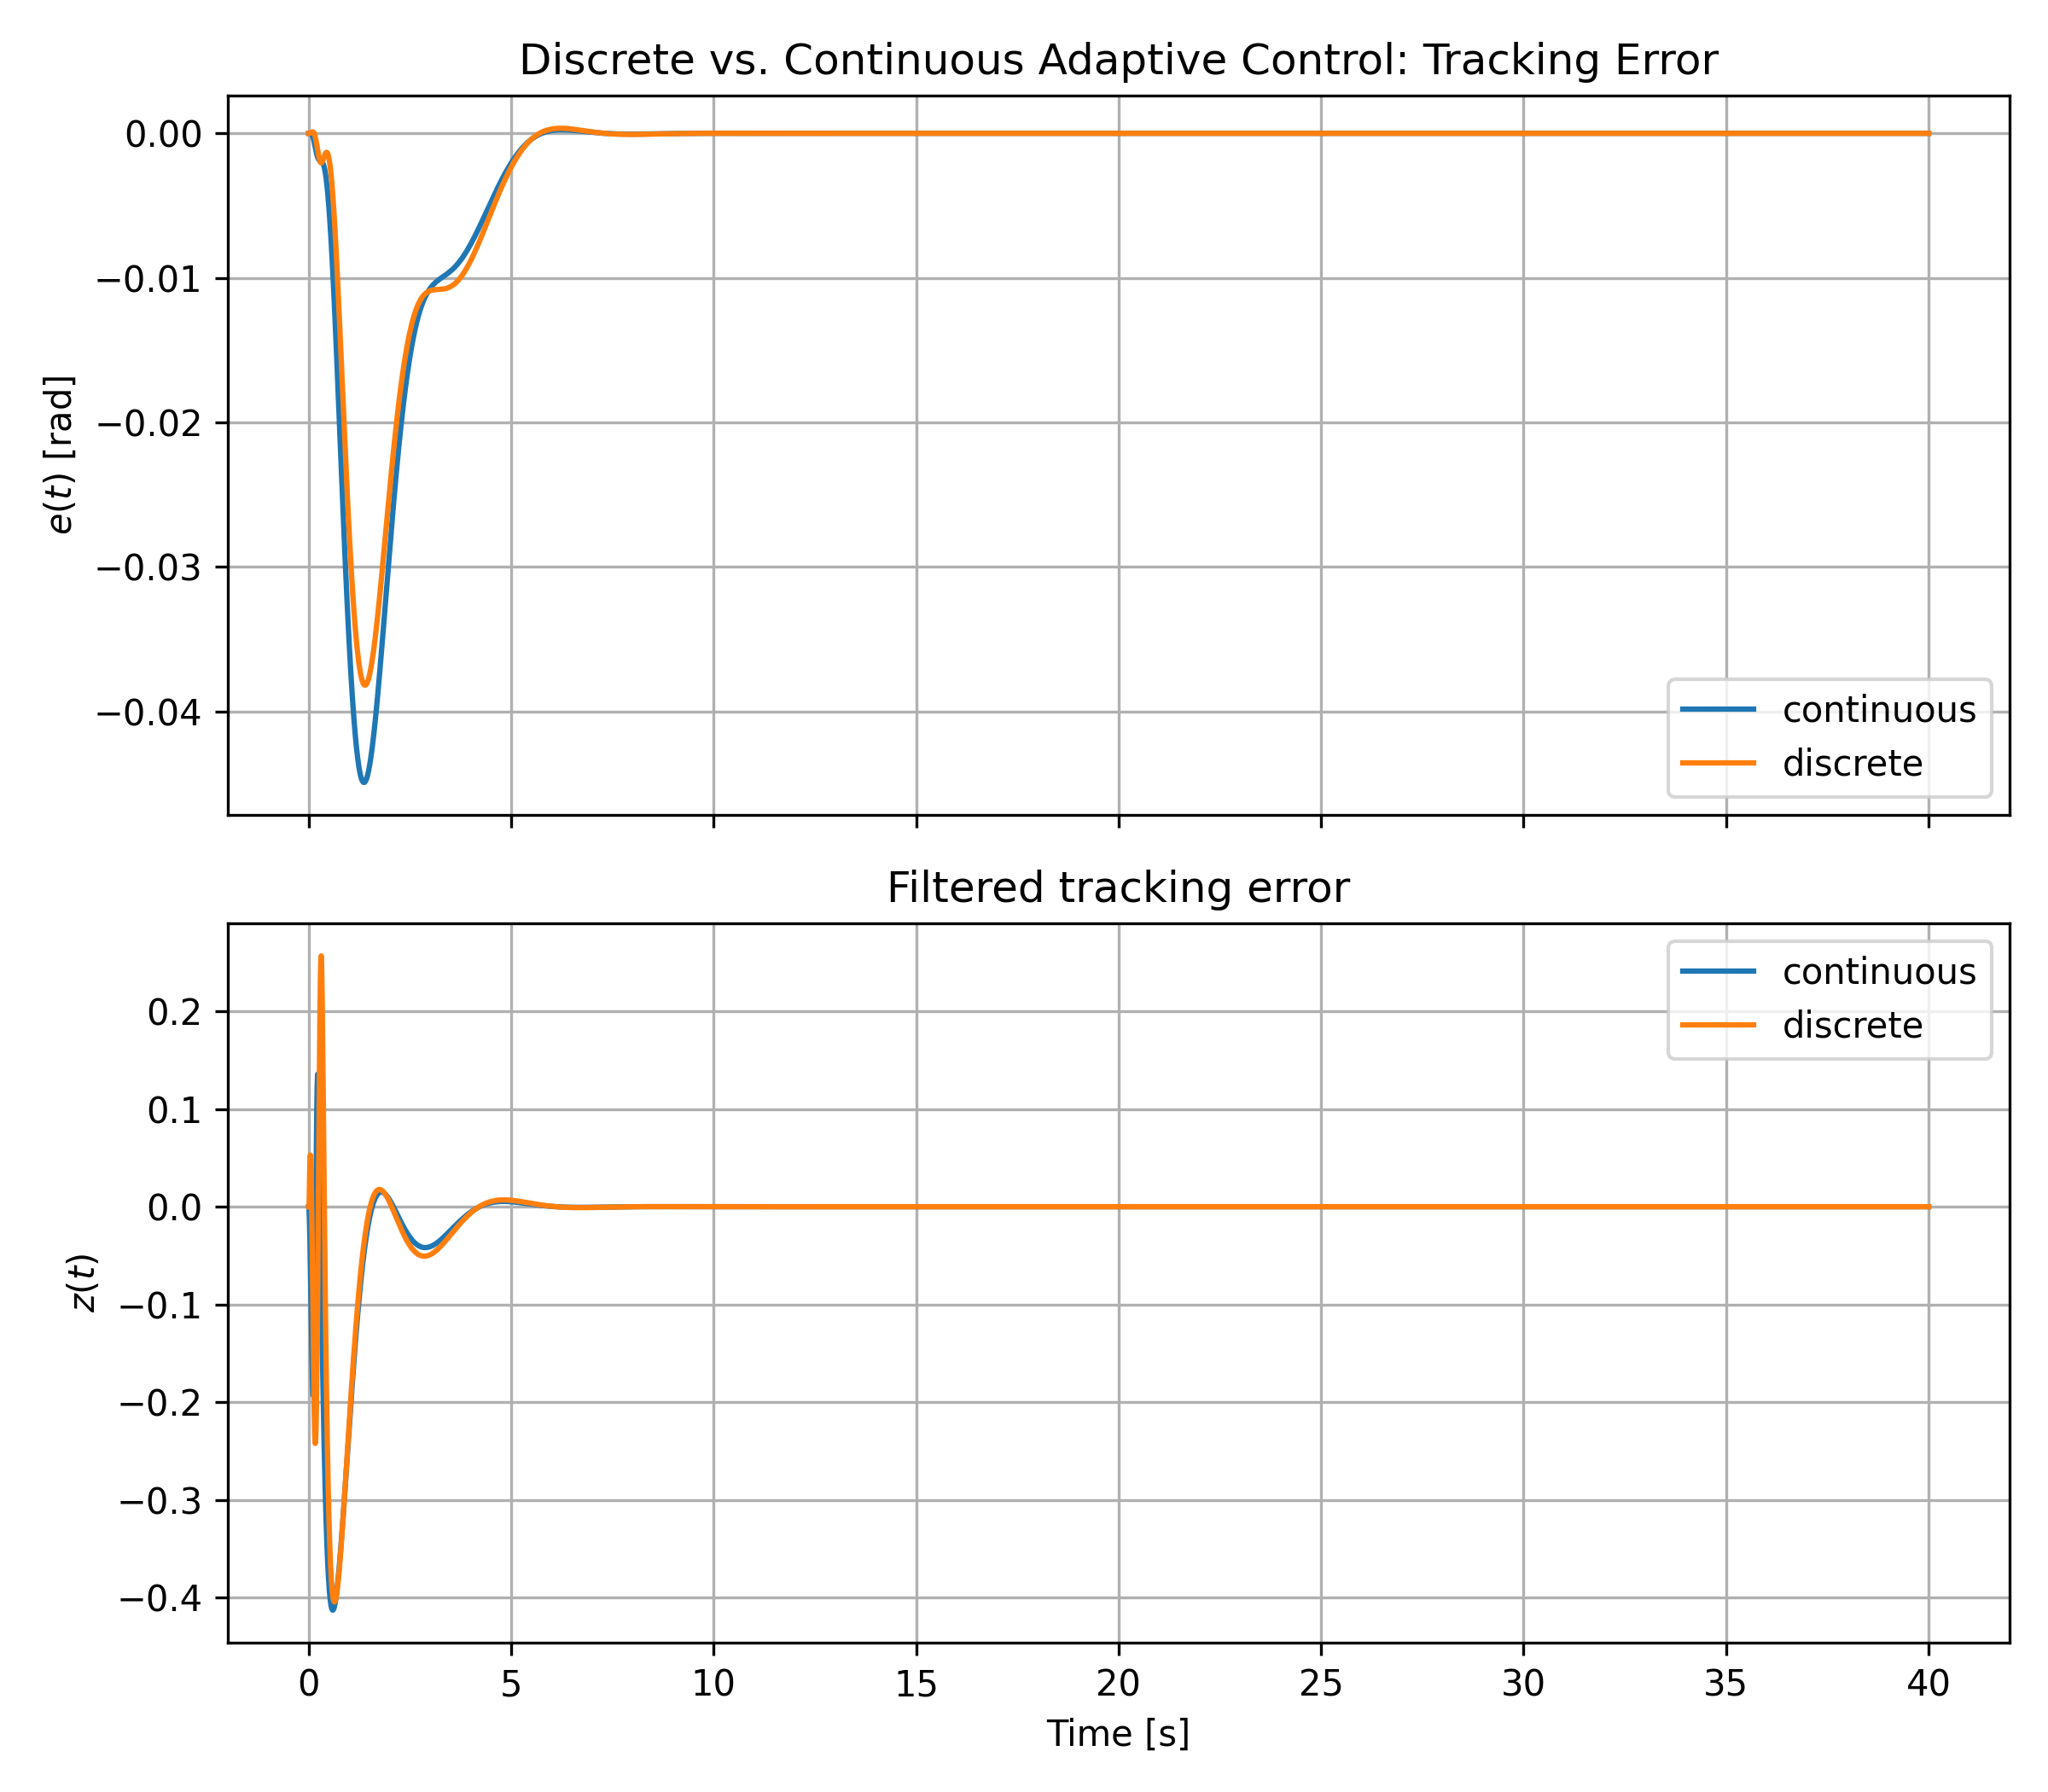
\includegraphics[width=0.7\textwidth]{figs/hw/section5_discrete_vs_continuous_errors.png}
\caption{Continuous-time vs. discrete-time tracking error \(e(t)\) (top) and filtered tracking error \(z(t)\) (bottom).}
\label{fig:discrete_errors}
\end{figure}

\begin{figure}[H]
\centering
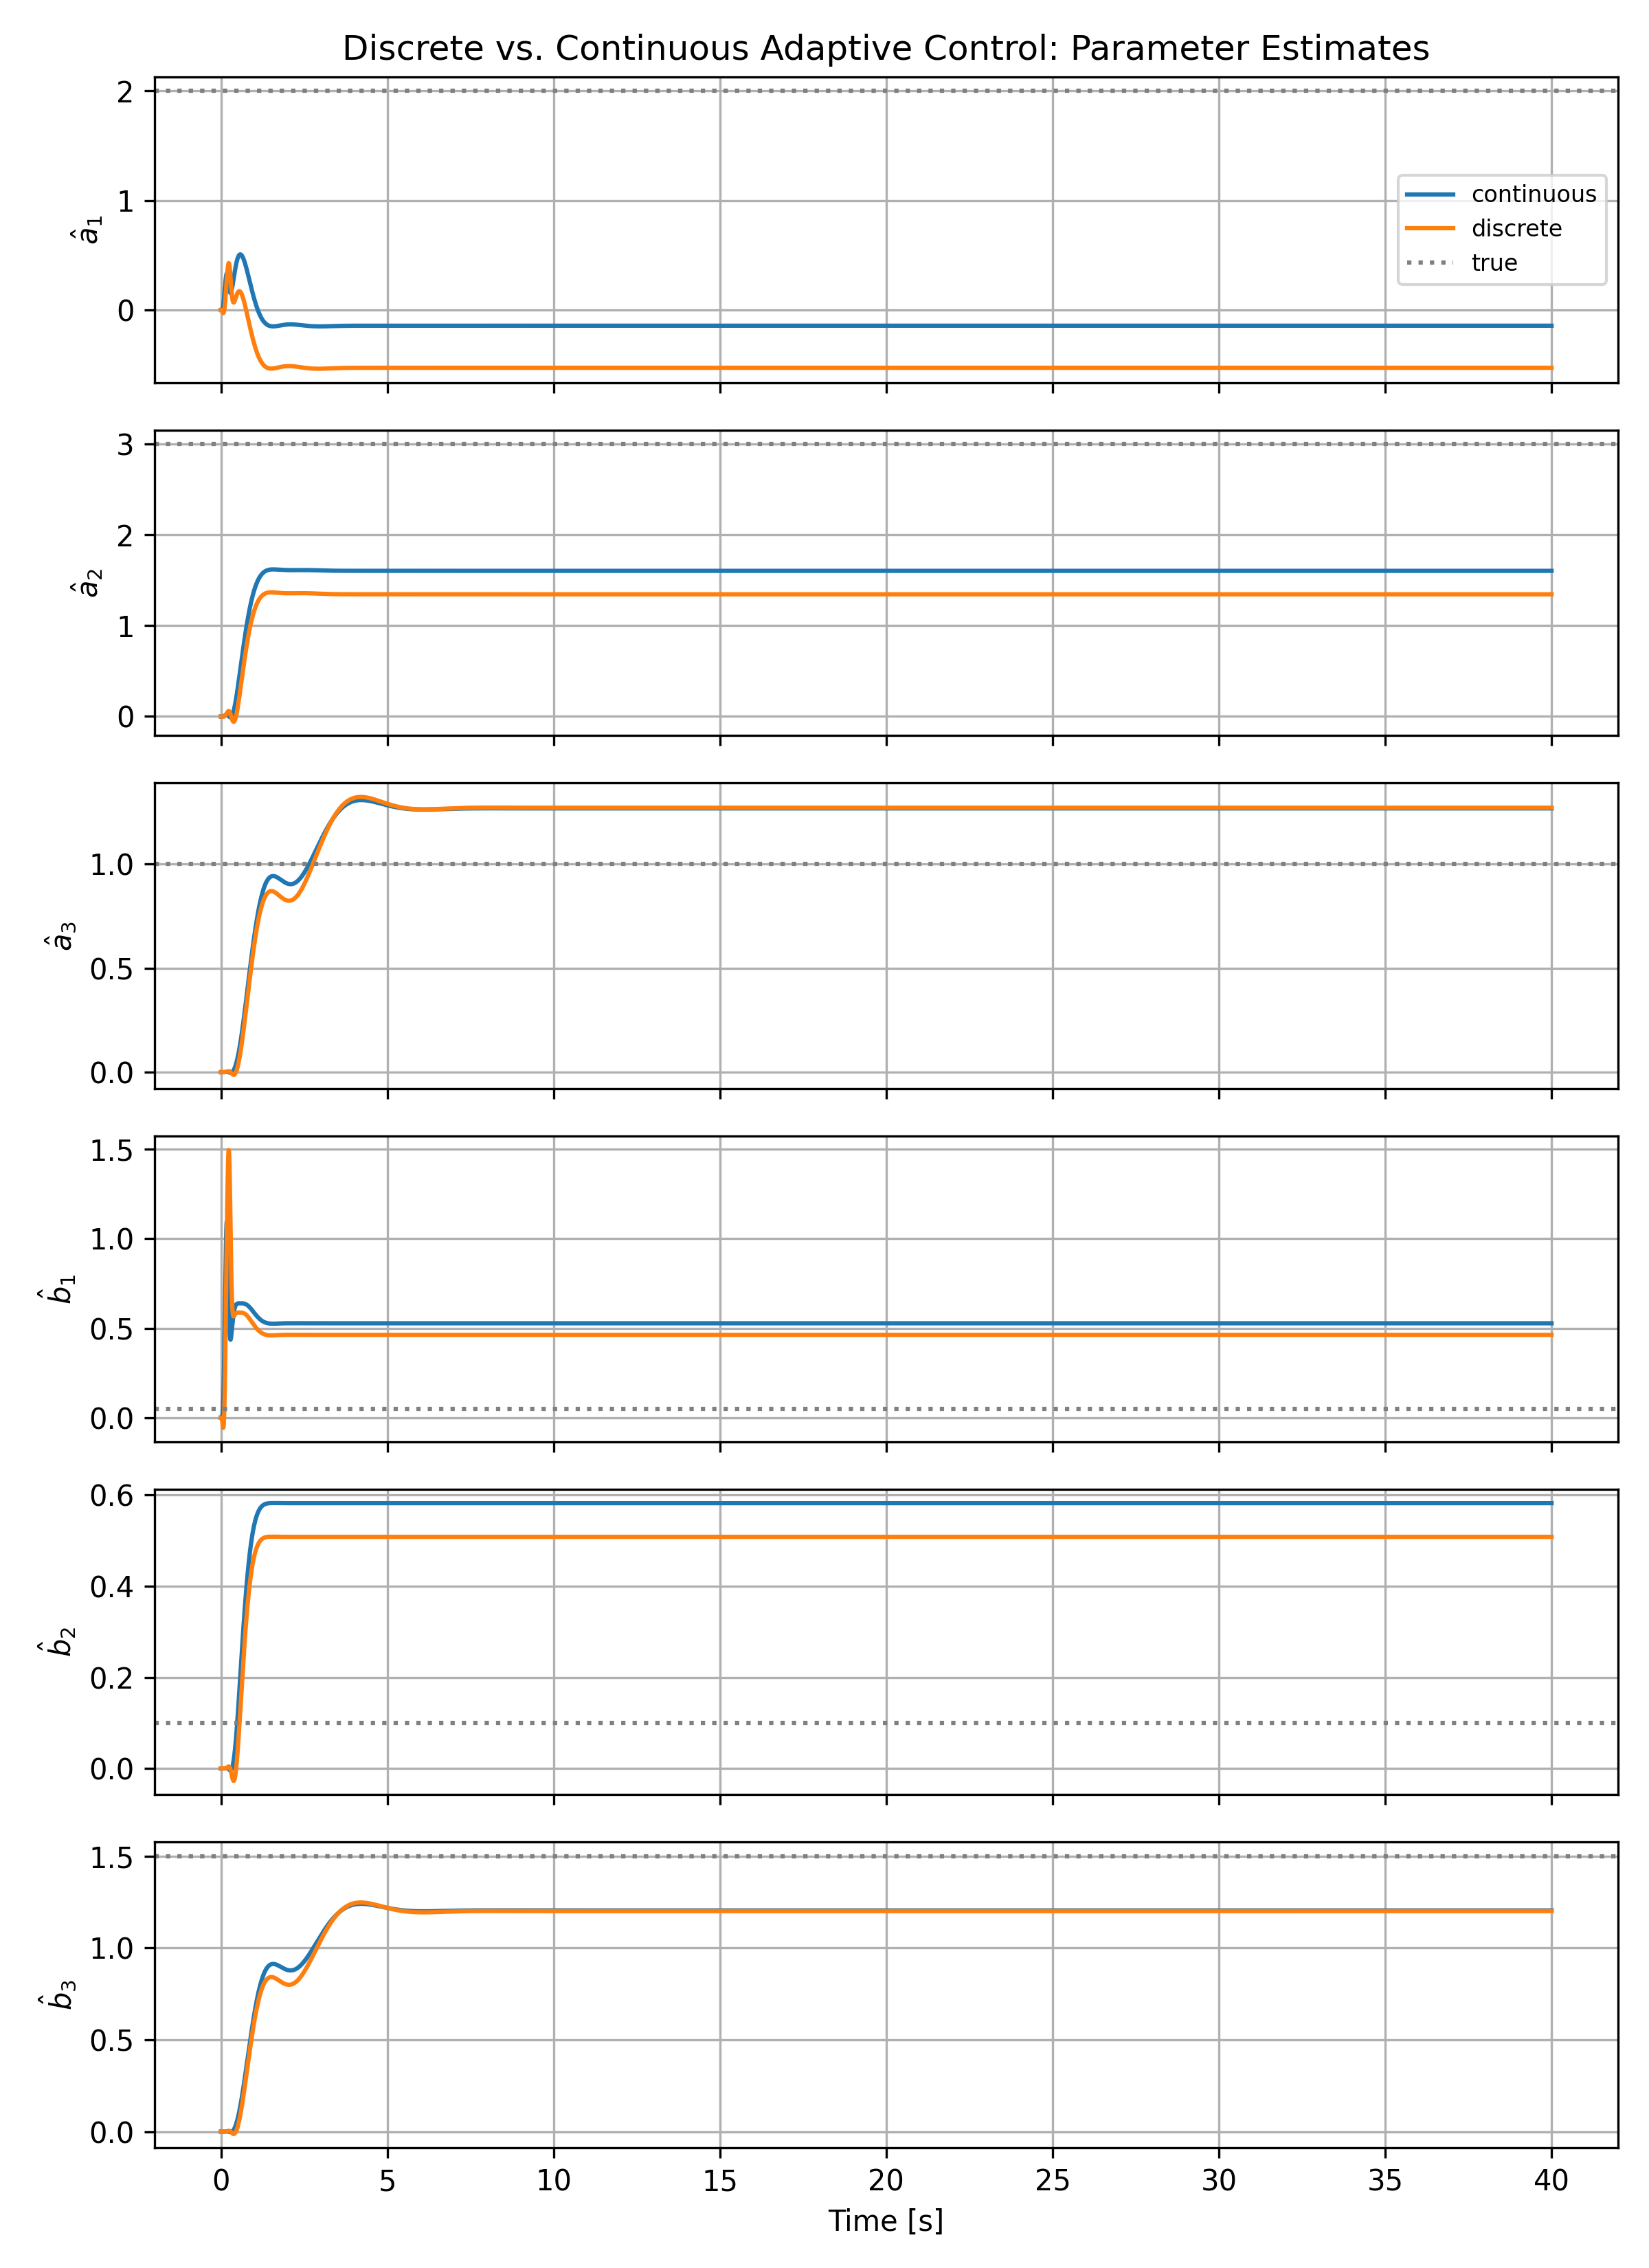
\includegraphics[width=0.7\textwidth]{figs/hw/section5_discrete_vs_continuous_parameters.png}
\caption{Parameter estimates \(\hat{\theta}_i(t)\): continuous-time vs. discrete-time.}
\label{fig:discrete_parameters}
\end{figure}

\noindent The discrete-time simulation shows that the adaptive controller can be implemented using recursive difference equations. The plant remains continuous-time, while the controller is updated once every sampling period and its output is held constant between samples.
For the selected sampling time \(T_s=0.01~\mathrm{s}\), the discrete-time controller achieves performance very similar to the continuous-time adaptive controller.
As in Section~4, the parameter estimates do not converge to their true values because the reference signal is a step input and does not provide sufficient excitation. Nevertheless, the parameter estimates remain bounded and the controller achieves accurate tracking.
The main advantage of this formulation is that it can be implemented directly on a microcontroller.

\bigskip